\chapter{Resultados experimentales} \label{cap:exp}
\section{Hist\'eresis en la medici\'on de rotaci\'on y elipticidad Kerr en una muestra de  CoFeB} \label{Exp:sec:hist}
Antes de intentar medir un espectro de efecto Kerr magneto-\'optico se desea observar ciclos de hist\'eresis los cuales son caracter\'isticos de materiales ferromagn\'eticos, \'este se midi\'o  con una longitud de onda de $660~nm$, lo cual equivale a una energ\'ia de fot\'on de $1.88~eV $. El campo magn\'etico externo se var\'ia entre los valores de $\pm 50~mT$, en donde el signo $\pm$ indica la direcci\'on del campo magn\'etico externo de acuerdo a lo descrito en la figura \ref{Met:fig:kerr}, lo que equivale de acuerdo a lo descrito en la sub secci\'on \ref{Met:subsec:Muest} en un campo magn\'etico $H$ en unidades c.g.s. de $\pm 500~ Oe$. En la figura \ref{Exp:fig:Kerrhis} se muestran las gr\'aficas de rotaci\'on (Fig. \ref{Exp:fig:theta}) y  elipticidad (Fig. \ref{Exp:fig:elip}) Kerr. En ambas gr\'aficas ya se aplic\'o la correcci\'on descrita por las ecuaciones \ref{Met:ec:divI1} y \ref{Met:ec:divI2}, es posible observar en ambas gr\'aficas un ciclo de Hist\'eresis en donde el cambio del \'angulo Kerr es de aproximadamente $0.2 ~mrad$ lo cual equivale a $0.0116 \degree$. En el caso de la elipticidad se obtiene una se\~nal de menor calidad pero s\'i es posible ver una tendencia: en este caso se puede detectar que el mayor cambio en la elipticidad es de $0.241~mrad$ que equivale a $0.0138 \degree$. Dicho valor muy parecido al obtenido con la rotaci\'on Kerr y  el campo de cohersi\'on $H_c$ con un valor aproximado de $\pm 100 ~Oe$.
\begin{figure}[!hbt]
	\centering
	\subfigure[Rotaci\'on Kerr]{
		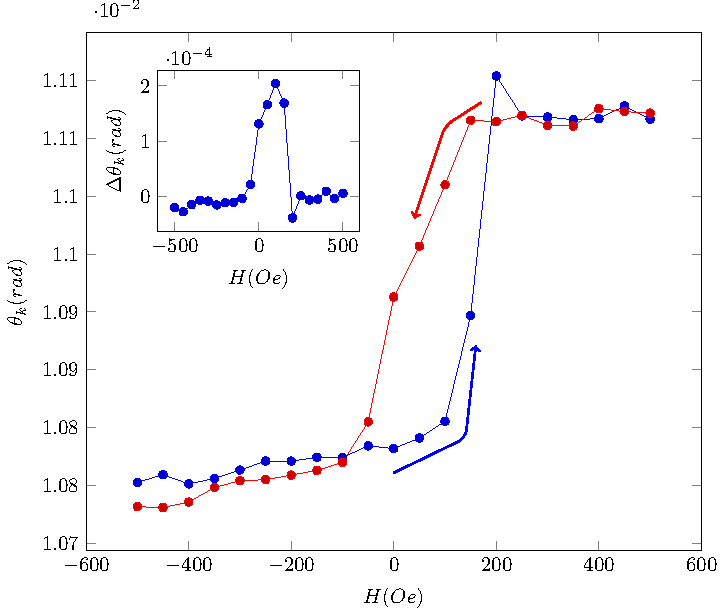
\includegraphics[scale=0.75]{resexp/his/HisTheta.pdf}
		\label{Exp:fig:theta}
	}
    \subfigure[Elipticidad Kerr]{
    	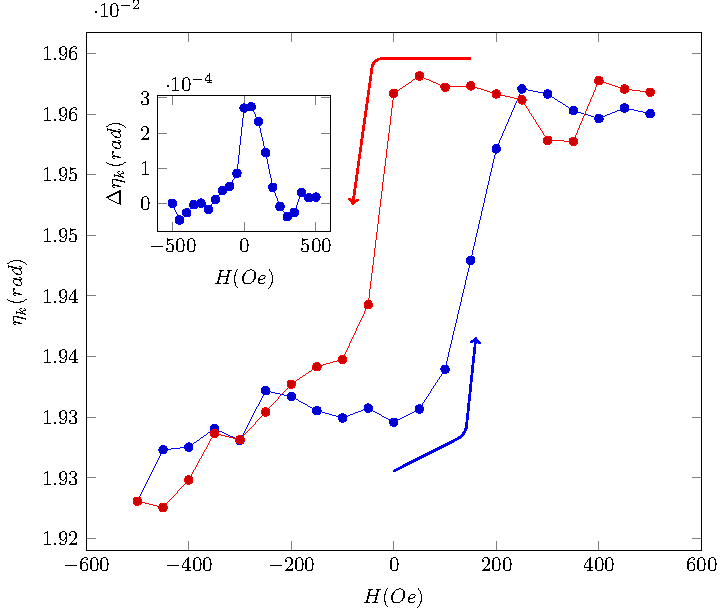
\includegraphics[scale=0.75]{resexp/his/HisEpsilon.pdf}
    	\label{Exp:fig:elip}
    }
 \caption[Hit\'eresis de $\theta_k$ y $\eta_k$ en CoFeB]{Medici\'on de rotaci\'on (\ref{Exp:fig:theta}) y elipticidad (\ref{Exp:fig:elip}) Kerr enuna muestra de CoFeB. Dentro de cada figura se muestra en cambio de la se\~nal medida con cada direcci\'on de campo magn\'etico.}
 \label{Exp:fig:Kerrhis}
  
\end{figure}
\newline
\section{Medici\'on de espectro de efecto Kerr mgneto-\'optico}
\par A continuaci\'on se utiliz\'o la fuente supercontinua y se midieron espectros con y sin campo magn\'etico aplicado y se obtuvieron los resultados que se muestran en la figura \ref{Exp:fig:espectroK}. En dicha figura es posible observar un cambio en el \'angulo y elipticidad Kerr; adem\'as se muestran la forma de linea que se obtiene cuando la referencia de $2f$ del lock in con respecto al campo magn\'etico corresponden las energ\'ias del fot\'on de $1.42 ~eV~y~1.48~eV$; adem\'as se observan ciclos de hist\'eresis lo cual indica que se est\'a midiendo un efecto magneto-\'optico en el CoFeB.
\begin{figure}[!hbt]
	\centering
	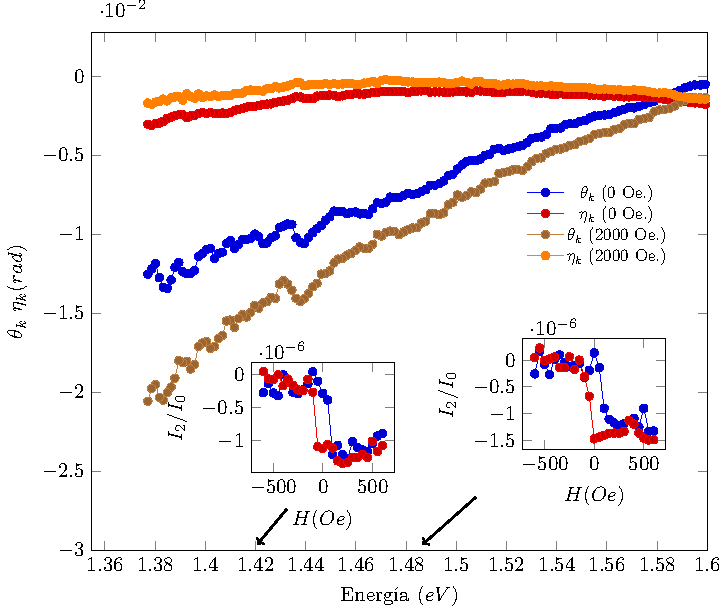
\includegraphics[scale=1]{resexp/esp/espectro0.pdf}
	\caption[Espectro de efecto Kerr magneto-\'optico]{Espectros del \'angulo y elipticidad Kerr en funci\'on de la energ\'ia del fot\'on en donde se induce un campo de $2000 Oe$.}
	\label{Exp:fig:espectroK}
\end{figure}
\newline
%\newline
\par En la figura  \ref{Exp:fig:difespectroK} se muestra la diferencia en $\theta_k$ y $\eta_k$ en donde se induce un campo de $2000 Oe$ y sin este. Es posible observar que si existen cambios entre estos y que rondan los $0.0015 ~rad$ para el caso de $\theta_k$ y de $-0.001 ~rad$ para $\eta_k$.
\begin{figure}[!hbt]
	\centering
	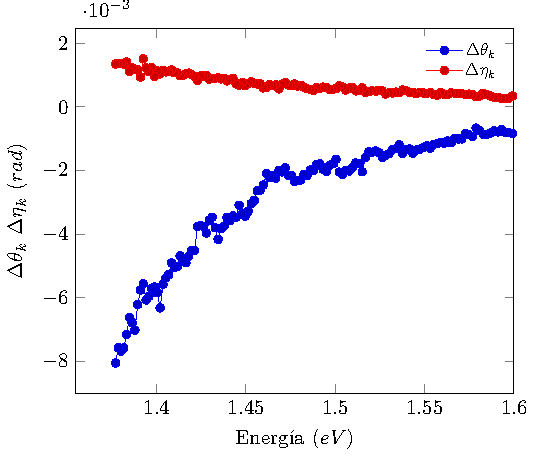
\includegraphics[scale=1.3]{resexp/esp/difespectro.pdf}
	\caption[Diferencia de mediciones de $\theta_k$ y $\eta_k$]{Diferencia en espectros del \'angulo y elipticidad Kerr en funci\'on de la energ\'ia del fot\'on.}
	\label{Exp:fig:difespectroK}
\end{figure}
Se ha comparado esta se\~nal con espectros obtenidos con otras configuraciones y se ha encontrado similitud entre \'estas \cite{Hoffmann_2019}. 
\endinput